\section{Servoberäkningar}

Servoberäkningarna tillkommer som underlag för objektidentifieringsdelen. Nedan behandlas samtliga beräkningar för de fyra servon som styr tummen och pekfingret. 

\subsection{Beräkningar för servo 1}

Servo 1 är med hjälp av ett stag kopplat till tummens första led och styr därmed dess $\alpha$ vinkel (se \ref{fig:servo1})

\begin{figure}[H]
\label{fig:servo1}
\includegraphics[width=0.4\textwidth]{img/servo/servo_berakning11}
\caption{Rörelse i tummens första led till följd av rörelse i servo 1}
\end{figure}

Bild \ref{fig:servo2} nedan visar hur servot är kopplat via ett stag till tummens första led. Servot har sin roterande axel i punkt $P_{0}$ vilken sedan är förskjutet till punkt $P_{1}$ med hjälp av ett servokors med radie $R_{1}$. Servokorset drar i sin tur i ett stag med längden c som påverkar tummens första led. Leden kan rotera kring punkt $P_{3}$ vilket ger upphov till en vinkel $\alpha$.


\begin{figure}[H]
\label{servo2}
\includegraphics[width=0.4\textwidth]{img/servo/servo1}
\caption{Nödvändiga beteckningar för beräkningar till servo 1}
\end{figure}

\[
\begin{cases}
r_{1}=\unit[16]{mm} \\
r_{2}=\unit[12]{mm}\\
a=\unit[4]{mm}\\
b=\unit[55]{mm}\\
c=\unit[58]{mm} \\
\end{cases}
\]

\begin{table}[H]
    \begin{tabular}{|c|l|l|}
        \hline
        Punkt  & X-Koordinat                          & Y-Koordinat                          \\ \hline
        $P_{0}$      & 0                                    & 0                                   \\ \hline
        $P_{1}$      & $r_{1}\cos(\phi)$              & $r_{1}\sin(\phi)$              \\ \hline
        $P_{2}$      & $P_{3x}-r_{2}\sin(\alpha)$                  & $P_{3y}+r_{2}\cos(\alpha)$                  \\ \hline
        $P_{3}$      & $b$ & $-a$ \\
        \hline
    \end{tabular}
\end{table}



Avståndet mellan punkterna $P_{2}$ och $P_{1}$ är  alltid c vilket är längden på staget som sammankopplar de båda punkterna. Detta utnyttjas för att upprätta ett itterations villkor. Ett gissat värde på alfa ($\alpha_{guess}$) ger koordinaterna för punkt $P_{2}$ vilket ger ett avstånd mha avståndsformeln (se itterationsschemat nedan). På så sät kan ett specifikt $\alpha$ fås för varje servo vinkel $\phi$

\begin{flushleft}

 (1)   $\phi,\alpha_{guess}$ $\rightarrow$ \\ 
  (2)  $P_{1}=[r_{1}\cos(\phi),r_{1}\sin(\phi)]$ $\rightarrow$
  \\(3) \thinspace $P_{2}=[P_{3x}-r_{2}\sin(\alpha_{guess}),P_{3y}+r_{2}\cos(\alpha_{guess})]$ $\rightarrow$ \\
  (4)\ $c_{g}=\sqrt[]{(P_{1x}-P_{2x})^2+(P_{1y}-P_{2y})^2}$ $\rightarrow$\\(5) Kolla om: $|c-c_{g}|>tol$ \\ (6) Om (5) stämmer $\rightarrow$ $\alpha_{guess}=\alpha_{guess}+value$ \ börja om från punkt (2) \\ \medspace annars \medskip $\rightarrow$ det approximativa $\alpha$-värdet har hittats
\end{flushleft}




